A naive classifier is the one which uses the true function $h(x)$ for classification. In this subsection, we compare the error made by the naive strategy with the deterministic and the stochastic Stackelberg equilibrium. We consider a scenario where the true function is $h(x)$ given in \eqref{eqn:True function}, $\up = \um := 2\uu$ where $\uu$ is sufficiently small and positive, the cost kernel is given by $\phi(x) = x$ and the probability law $D \in \fk{D}$ is uniform.

In the first example, we calculate the error made by the naive classifier.
\begin{exg}\label{eg:naive}
	The naive classifier $h(x)$ is given by

	\begin{equation*}
		\begin{aligned}
			h(x) = \begin{cases}
				\minus&  x \in [0,\h] \\

				\plus &  x \in (\h,1].\\
			\end{cases}
		\end{aligned}
	\end{equation*}
For a feature vector $x \in (\h - 2\uu, \h]$, the sender can map it to a feature vector $x'$, where $x'$ is such that $\h < x' < x + 2\uu$, and obtain a positive payoff. This is better than not modifying $x$, as in that case, the sender receives zero payoff.
Similarly, for a feature vector $x \in (\h, \h + 2\uu]$, the sender can map it to a feature vector $x'$, where $x'$ is such that $x - 2\uu < x' \leq \h$, and obtain a positive payoff as opposed to a zero payoff when not modifying $x$. Hence $h(x)$ misclassifies the feature vectors belonging in the interval $(\h-2\uu,\h+2\uu]$ and $\cg{E}(h) = 4\uu$.

	\begin{figure}
		\centering
		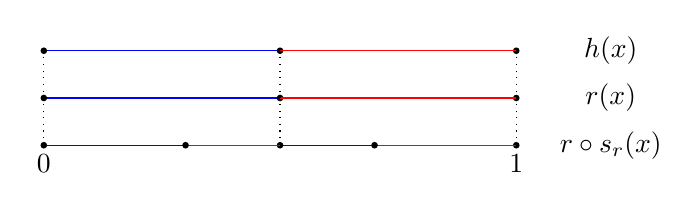
\begin{tikzpicture}[scale=0.6]
			% Blue horizontal line
			\draw[blue] (0,1) -- (5,1);
			\draw[blue] (0,0) -- (5,0);
			\draw[blue] (5,-1) -- (7,-1);
			\draw[blue] (0,-1) -- (3,-1);
			\fill[black] (5,0) circle (2pt);
			\fill[black] (0,0) circle (2pt);
			\fill[black] (10,0) circle (2pt);
			\fill[black] (5,1) circle (2pt);
			\fill[black] (0,1) circle (2pt);
			\fill[black] (10,1) circle (2pt);
			\fill[black] (0,-1) circle (2pt);
			\fill[black] (10,-1) circle (2pt);
			\fill[black] (5,-1) circle (2pt);
			\node[below] at (3,-1) {$\hminus$};
			\node[above] at (2.5,1) {$\minus$};
			\node[above] at (2.5,0) {$\minus$};
			\node[above] at (1.5,-1) {$\minus$};
			\node[above] at (6,-1) {$\minus$};

			% Red horizontal line
			\draw[red] (5,1) -- (10,1);
			\draw[red] (5,0) -- (10,0);
			\draw[red] (3,-1) -- (5,-1);
			\draw[red] (7,-1) -- (10,-1);
			\fill[black] (3,-1) circle (2pt);
			\fill[black] (7,-1) circle (2pt);
			\node[below] at (7,-1) {$\hplus$};
			\node[above] at (7.5,1) {$\plus$};
			\node[above] at (7.5,0) {$\plus$};
			\node[above] at (4,-1) {$\plus$};
			\node[above] at (8.5,-1) {$\plus$};

			\draw[black,dotted] (0,1) -- (0,-1);
			\draw[black,dotted] (5,1) -- (5,-1);
			\draw[black,dotted] (10,1) -- (10,-1);
			\node[below] at (0,-1) {$0$};
			\node[below] at (10,-1) {$1$};
			\node[below] at (5,-1) {$\h$};
			\node at (12,0) {$r(x)$};
			\node at (12,-1) {$r \circ s_r(x)$};
			\node at (12,1) {$h(x)$};
		\end{tikzpicture}
        \caption{Naive classifier.}
	\end{figure}
\end{exg}


In the next example, we calculate the error made by the deterministic Stackelberg equilibrium.
\begin{exg}	Let $r^*$ be a deterministic Stackelberg equilibrium obtained from Theorem \ref{thm:Deterministic Stackelberg equilibrium strategy}. Then $r^*$ is given by

	\begin{equation*}
		\begin{aligned}
			r^*(x) = \begin{cases}
				h(x) & \text{if } x \in [0,\hminus) \cup (\hplus,1]\\
				\Delta & \text{if } x \in [\hminus,\hplus],
			\end{cases}
		\end{aligned}
	\end{equation*}
	where $\hminus = \h - \uu$ and $\hplus = \h + \uu$. The sender's worst-case best response is
	\begin{equation*}
		\begin{aligned}
			s_{r^*}(x) = \begin{cases}
				x & \text{if } x \in [0,\hminus) \cup (\hplus,1]\\\
				\hplus & \text{if } x \in [\hminus,\h) \\
				\hminus & \text{if } x \in [\h,\hplus].
			\end{cases}
		\end{aligned}
	\end{equation*}
Hence $E(r^*) = [\hminus,\hplus]$ and $\cg{E}(r^*) = 2\uu$. This shows that ignoring feature vectors near the decision boundaries, which in any case will be misclassified under the naive decision rule, prevents other neighbouring feature vectors from getting misclassified.
	\begin{figure}
		\centering
		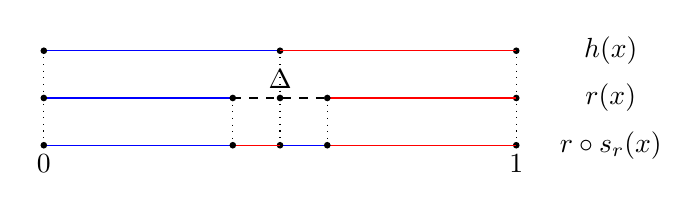
\begin{tikzpicture}[scale=0.6]
			% Blue horizontal line
			\draw[blue] (0,1) -- (5,1);
			\draw[blue] (0,0) -- (4,0);
			\draw[blue] (5,-1) -- (6,-1);
			\draw[blue] (0,-1) -- (4,-1);
			\fill[black] (5,0) circle (2pt);
			\fill[black] (0,0) circle (2pt);
			\fill[black] (10,0) circle (2pt);
			\fill[black] (5,1) circle (2pt);
			\fill[black] (0,1) circle (2pt);
			\fill[black] (10,1) circle (2pt);
			\fill[black] (0,-1) circle (2pt);
			\fill[black] (10,-1) circle (2pt);
			\fill[black] (5,-1) circle (2pt);
			\node[below] at (4,-1) {$\hminus$};
			\node[above] at (2.5,1) {$\minus$};
			\node[above] at (2.5,0) {$\minus$};
			\node[above] at (2,-1) {$\minus$};
			\node[above] at (5.5,-1) {$\minus$};

			% Red horizontal line
			\draw[red] (5,1) -- (10,1);
			\draw[red] (6,0) -- (10,0);
			\draw[red] (4,-1) -- (5,-1);
			\draw[red] (6,-1) -- (10,-1);
			\fill[black] (4,0) circle (2pt);
			\fill[black] (6,0) circle (2pt);
			\fill[black] (4,-1) circle (2pt);
			\fill[black] (6,-1) circle (2pt);
			\node[below] at (6,-1) {$\hplus$};
			\node[above] at (7.5,1) {$\plus$};
			\node[above] at (7.5,0) {$\plus$};
			\node[above] at (4.5,-1) {$\plus$};
			\node[above] at (8,-1) {$\plus$};
			\node[above] at (5,0) {$\Delta$};


			\draw[dashed] (4,0) -- (6,0);
			\draw[black,dotted] (0,1) -- (0,-1);
			\draw[black,dotted] (5,1) -- (5,-1);
			\draw[black,dotted] (10,1) -- (10,-1);
			\draw[black,dotted] (4,0) -- (4,-1);
			\draw[black,dotted] (6,0) -- (6,-1);
			\node[below] at (0,-1) {$0$};
			\node[below] at (10,-1) {$1$};
			\node[below] at (5,-1) {$\h$};
			\node at (12,0) {$r(x)$};
			\node at (12,-1) {$r \circ s_r(x)$};
			\node at (12,1) {$h(x)$};
		\end{tikzpicture}
        \caption{Deterministic Stackelberg equilibrium.}
	\end{figure}
\end{exg}

In Section \ref{subsec:Deterministic strategy}, we analyzed the setup where the sender adopts the worst-case best response. In contrast, Section \ref{subsec:Stochastic strategy} examined the setup where the sender employs the worst-case lazy best response. To ensure a fair comparison between the deterministic and stochastic Stackelberg equilibria, the sender's style of play should remain fixed. Therefore, in the following example, we calculate the classification error made by a receiver strategy, assuming the sender adopts the worst-case best response.


\begin{exg}\label{ex:eps stochastic strategy}
Let $\eps >0 $. Let $r_\eps \equiv (1-q_\eps(x),q_{\eps}(x),0)$ be stochastic receiver strategy where $q_\eps$ is defined as \begin{equation}\label{eqn:q eps formula}
		q_\eps(x) = \begin{cases}
			0 & \text{if } x \in [0,\hminuseps) \\
			\frac{x-\hminuseps}{2(\uu + \eps)}& \text{if } x \in [\hminuseps,\hpluseps]\\
		  1 & \text{if } x \in (\hpluseps,1],
		\end{cases}
	\end{equation}
where $\hminuseps := \h - \uu - \eps$ and $\hpluseps := \h + \uu + \eps$.
It follows that the worst-case best response is $s_{r_\eps}(x) = x$ (the calculation is similar to what is done in Lemma \ref{lem:error is half} and is given in Section~\ref{sec:proofs_ch2}, Calculation~\ref{cal:eps stochastic strategy}) and $\cg{E}(r_\eps)$ is $\frac{\uu + \eps}{2}$. This strategy shows that randomizing classifications near the decision boundaries can correctly classify feature vectors close to the decision boundaries, albeit with a low but positive probability. This happens because randomization ensures that the cost increase is offset by the increase in utility (which takes a fractional value due to randomization).
    \begin{figure}
		\centering
		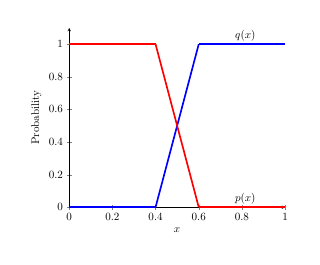
\begin{tikzpicture}[scale=0.4]
			\begin{axis}[
				axis lines = left,
				xlabel =$x$,
				ylabel = {Probability},
				xmin = 0,
				xmax = 1,
				ymin = 0,
				ymax = 1.1,
				legend pos = north west,
				]

				% Piecewise function q_{\eps}(x)
				\addplot[
				domain=0:0.4,
				samples=100,
				color=blue,
				line width=2.5pt,
				]{0};
				\addplot[
				domain=0.4:0.6,
				samples=100,
				color=blue,
				line width=1.5pt,
				]{5 * (x - 0.4)};
				\addplot[
				domain=0.6:1,
				samples=100,
				color=blue,
				line width=1.5pt,
				]{1};

				% Piecewise function p(x)
				\addplot[
				domain=0:0.4,
				samples=100,
				color=red,
				line width=1.5pt,
				]{1};
				\addplot[
				domain=0.4:0.6,
				samples=100,
				color=red,
				line width=1.5pt,
				]{-5*(x)+3};
				\addplot[
				domain=0.6:1,
				samples=100,
				color=red,
				line width=2.5pt,
				]{0};

				% Add labels
				\node[right] at (axis cs: 0.35,0.2) {};
				\node[right] at (axis cs: 0.5,0.7) {};
				\node[right] at (axis cs: 0.75,1.05) {$q_{\eps}(x)$};
				\node[right] at (axis cs: 0.75,-0.2) {};
				\node[right] at (axis cs: 0.5,-0.7) {};
				\node[right] at (axis cs: 0.75,0.05) {$p(x)$};

			\end{axis}
		\end{tikzpicture}
		\caption{Stochastic decision rule$r(x)$,$\uu = 0.1$,$\h = 0.5$}
		\label{fig:Stochasticdecisionrule}
	\end{figure}
\end{exg}

It can be seen from these examples that both the deterministic and stochastic Stackelberg equilibria outperform the naive classifier. Furthermore, the stochastic classifier makes fewer errors than the deterministic classifier. The benefit of randomization in strategic interactions is well-established in game theory literature, and we now observe its advantages in the strategic classification as well.

One crucial point to note is that although the penalty label was useful in the deterministic classifier, it was not helpful in the stochastic classifier. Furthermore, the deterministic classifier is sub-optimal compared to the stochastic classifier. Thus, the randomization offers the receiver a richer source of leverage to make the sender behave appropriately than the penalty label. However, in many cases, such as university admissions, for transparency, the receivers are constrained to use only the deterministic classifier. Thus, in those cases, the penalty label can act as compensation for the lack of randomization.

The following example describes the deterministic Stackelberg equilibrium of the university admission problem introduced in the Section \ref{sec:Introduction}.

\begin{exg}(Stackelberg equilibrium of the university admission problem):\\

Recall the example from the introduction. Suppose a university offers two programs: Theoretical Physics and Experimental Physics. Admission to these programs is determined by each student’s performance on an entrance exam. Each prospective student has a unique combination of theoretical and experimental skills, and their \textit{true program} corresponds to the program that aligns with their stronger skill. However, students often prefer a program that does not align with their true program. The university’s goal is to design the entrance exam to maximize the number of students admitted to their true program.

We model this as a strategic classification problem as follows: The university acts as the receiver, and the student as the sender. Let $\cg{X} := [0,1]$ represent the set of feature vectors, where $x \in \cg{X}$ denotes a student's true aptitude, with the interpretation that it has $x$ theoretical skill and $(1 - x)$ experimental skill. We assume that true aptitudes are uniformly distributed across the student population; thus, $D$, the probability law on $\cg{X}$, is uniform. Let $\cg{Y} := \{\minus,\plus\}$ denote the label space, where $\minus$ indicates the Experimental Physics program and $\plus$ the Theoretical Physics program. The true function $h(x)$, which assigns each student to their true program, is given by the following equation:
\begin{equation}
    h(x) = \begin{cases}
    \plus & \text{if } x > 0.5, \\
    \minus & \text{if } x \leq 0.5.
    \end{cases}
\end{equation}
This means $\h = 0.5$, and that for $x > 0.5$, a student’s true program is Theoretical Physics, while for $x \leq 0.5$, it is Experimental Physics.

The university has access to a question bank containing questions of varying difficulties. We denote the difficulty level of a question by $x$, indicating that the question requires $x$ theoretical knowledge and $(1 - x)$ experimental knowledge to solve. Note that there is a one-to-one correspondence between the feature vector set $\cg{X}$ and the question bank. Thus, a student may demonstrate an aptitude $x'$ (not necessarily their true aptitude) by solving a question with difficulty level $x'$. The entrance exam comprises multiple questions selected from this bank, with each question associated with a program. A student can attempt only one question, and admission to the corresponding program is granted if they answer correctly.

We assume each student's preferred program differs from their true program. The student’s utility function is given by
\begin{equation}
	U(y,x) := \begin{cases}
		0.04 & x \in [0,0.5], y = \plus \\
		0.04 & x \in (0.5,1], y = \minus \\
		0 & y = h(x)\\
		-\infty & y = \Delta.
	\end{cases}
\end{equation}
This means $\um = \up = 0.04$ , and a student gains a utility of $0.04$ if assigned to their preferred program and $0$ if assigned to their true program and $-\infty$ if not assigned any program. The cost kernel is given by $\phi(x) = x$, meaning that for a question with difficulty level $x'$, a student with true aptitude $x$ incurs a cost of $|x - x'|$ while solving it.

The university's strategy set includes all possible question papers for the entrance exam. For a given question paper, each student selects the question that maximizes their utility at the lowest cost, potentially demonstrating an aptitude $x'$ different from their true aptitude to the university. The student’s strategy set consists of mappings that specify which question to attempt for each question paper. We assume students answer their chosen question correctly. Consequently, the university, aware of students' strategic behaviour, must optimally design the question paper to maximize the number of students admitted to their true program.

According to Theorem \ref{thm:Deterministic Stackelberg equilibrium strategy}, questions with difficulty levels in the interval $[\h- \um,\h+\up]$ should not be included in the exam. Substituting the value for  $\h,\um,\up$ for this example, this interval turns out to be $[0.48,0.52]$. Furthermore, the students who correctly answers questions with difficulty levels less than $0.48$ should be admitted to the Experimental Physics program, and the students who correctly answers the questions with difficulty levels greater than $0.52$ should be admitted to the Theoretical Physics program. The intuition for excluding questions in the interval $[0.48,0.52]$ is as follows: if a question of difficulty level, say $0.51$ (corresponding to Theoretical Physics) is included, a student with true aptitude $0.49$ (whose true program is Experimental Physics) could solve it with only effort $0.02$, leading to misclassification. However, this approach has a drawback: students whose true aptitudes lie within the interval $[0.48,0.52]$ must attempt questions of difficulty level outside this range. Thus, by incurring a cost, they attempt questions linked to their preferred program and get misclassified by the university. Nonetheless, the overall benefits of this strategy outweigh its drawbacks, making it the optimal option for the university.

\end{exg}


\subsection{Other Stackelberg equilibria}\label{subsec:Other equilibria}
In this section, we only consider deterministic Stackelberg equilibria. In many scenarios, the strategic classification problem may admit more than one Stackelberg equilibrium. While all such Stackelberg equilibria guarantee the same classification error for the receiver, they are not equivalent from the sender's perspective. Here, we discuss various considerations that a receiver may take into account besides minimizing the classification error.

\subsubsection{Participation constraint for the sender}
Consider the following instance of the problem. Let $D$ be a uniform distribution on $\cg{X}$, with $\h = 0.5$ and $\um = \up = 0.1$. It can be shown that both $r_1$ and $r_2$, defined as
\begin{equation*}
r_1(x) = \begin{cases}
\minus & \text{if } x \in [0, 0.45] \\
\Delta & \text{if } x \in (0.45, 0.55) \\
\plus & \text{if } x \in [0.55, 1]
\end{cases}, \;\;\;\;
r_2(x) = \begin{cases}
\minus & \text{if } x = 0 \\
\Delta & \text{if } x \in (0, 1) \\
\plus & \text{if } x = 1
\end{cases}
\end{equation*}
are receiver Stackelberg equilibrium strategies. However, the situation differs from the sender's perspective. For $x \in \cg{X}$, the sender's payoff under $r_1$ and $r_2$ satisfies
\begin{equation}
\mathbb{U}(x; r_1, s_{r_1}) \geq \mathbb{U}(x; r_2, s_{r_2}) \text{ for all } x \in \cg{X}.
\end{equation}
That is, for each $x \in \cg{X}$, the payoff for the sender under $r_1$ is greater than or equal to that under $r_2$.

This scenario resembles a dilemma in the principal-agent problem, where the principal can impose an unfair contract on the agent, who ends up paying (instead of being paid) for their work. To remedy this in the principal-agent context, the agent is given the option to refuse the contract and receive a baseline payoff. This encourages the principal to offer a contract with a payoff greater than the baseline. This concept is known as the \textit{participation constraint} for the agent.

Drawing a parallel to the principal-agent problem, the receiver can be viewed as the principal who offers a contract $r$, while the sender acts as the agent who, by making effort $s$ on a feature vector $x$, gets a payoff of $\mathbb{U}(x; r, s)$. We allow the sender, after seeing the contract $r$, the option not to participate and instead receive a baseline payoff. There are many ways the sender can determine his decision to participate. Here, we assume that the sender does not participate if $\mathbb{U}(x; r, s_r)$ is lower than the baseline payoff for any $x \in \cg{X}$. We further assume that if the sender does not participate in the game, the receiver makes an error on the entire $\cg{X}$. This participation constraint of the sender would discourage the receiver from playing a degenerate strategy like $r_2$, since the sender would reject such a game. Given this constraint, strategies like $r_1$, with a $\Delta$ interval of length $\uu$, provide justifiable non-degenerate Stackelberg equilibria, as we show in the following cases.


\noindent \textit{Case 1 (Negative participation constraint): }\\
Suppose the sender incurs a fixed payoff $\nu \leq 0$ if it chooses not to participate in the game after seeing the receiver's strategy. This means the sender can opt-out with a small penalty upon encountering an unfavourable receiver strategy. Consequently, many degenerate receiver strategies like $r_2$ will not satisfy the participation constraint and will no longer be a receiver Stackelberg equilibrium.

Now consider the strategy $r_1$. For $x \in [0, 0.45) \cup (0.55, 1]$, the sender's payoff at $x$ is $\mathbb{U}(x; r, s_r) = 0$. For $x \in [0.45, 0.5]$, the sender's payoff at $x$ is $\mathbb{U}(x; r, s_r) = x - 0.45$ and for $x \in (0.55, 1]$, the sender's payoff at $x$ is $\mathbb{U}(x; r, s_r) = 0.55 - x$. Thus, $\min_{x \in \cg{X}} \mathbb{U}(x; r, s_r) = 0$. This satisfies the sender's participation constraint, and hence the sender will participate in the game. Therefore, $r_1$ is a Stackelberg equilibrium even under this constraint.

\noindent \textit{Case 2 (Positive participation constraint): }\\
Suppose the sender receives a fixed payoff $\nu > 0$ if it chooses not to participate in the game after seeing the receiver's strategy. We will show that every receiver strategy is a Stackelberg equilibrium strategy.

Let $r$ be a receiver strategy. If $E(r, s_r, h) = \cg{X}$, then $\cg{E}(r) = 1$. If $E(r, s_r, h) \neq \cg{X}$, then there exists $x$ such that $r(s_r(x)) = h(x)$. This implies $\mathbb{U}(x; r, s_r) = -|s_r(x) - x| \leq 0$. But this violates the sender's participation constraint, and thus the sender will ignore this strategy $r$. Therefore, $\cg{E}(r) = 1$. Hence, $\cg{E}(r) = 1$ for all $r \in \msf{R}$. Therefore, every receiver strategy $r \in \msf{R}$ is a receiver Stackelberg equilibrium strategy as claimed. More specifically, $r_1$ is a Stackelberg equilibrium even under this constraint.


\subsubsection{Fairness and complexity of the classifier:}
Let $D$ be the uniform probability law on $[0,1]$, $\h = 0.5$, and $\um = \up = 0.1$. From Theorem \ref{thm:Deterministic Stackelberg equilibrium strategy}, any strategy $r(x; \hminus, \hplus) \in \sr{R}$ such that $\hminus \leq 0.5 \leq \hplus$ and $|\hminus - \hplus| = 0.1$ is a Stackelberg equilibrium. These equilibria yield the same receiver error but differ in how errors are distributed across each label class.

Consider two such receiver strategies, $r_1$ and $r_2$, with 
corresponding $\Delta$-regions $(0.45, 0.55)$ and $(0.4, 0.5)$, 
respectively. The strategy $r_1$ appears fairer, as it balances 
the ratio of correctly classified labels, compared to $r_2$, 
which misclassifies only the $-$ class. However, the receiver 
strategy $r_2$ is simpler, with 2 decision boundaries in 
$r_2 \circ s_{r_2}$ compared to 3 in $r_1 \circ s_{r_1}$. 
This simplicity is an advantage for learnability; 
the VC dimension of a hypothesis class increases with the number of decision 
boundaries that functions in that class are allowed to have
(see Proposition \ref{prop: VC dimension}). This 
highlights a trade-off between fairness and 
efficient learnability. Depending on the 
application, one strategy may be preferable to the other.

\begin{figure}
		\centering
		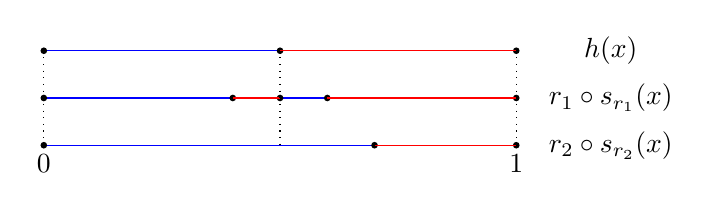
\begin{tikzpicture}[scale=0.6]
			% Blue horizontal line
			\draw[blue] (0,1) -- (5,1);
			\draw[blue] (0,0) -- (4,0);

                \draw[blue] (5,0) -- (6,0);
			\draw[blue] (0,-1) -- (7,-1);
			\fill[black] (4,0) circle (2pt);
                \fill[black] (6,0) circle (2pt);
                \fill[black] (5,0) circle (2pt);
			\fill[black] (0,0) circle (2pt);
			\fill[black] (10,0) circle (2pt);
			\fill[black] (5,1) circle (2pt);
			\fill[black] (0,1) circle (2pt);
			\fill[black] (10,1) circle (2pt);
			\fill[black] (0,-1) circle (2pt);
			\fill[black] (10,-1) circle (2pt);
			\fill[black] (7,-1) circle (2pt);

			\node[above] at (2.5,1) {$\minus$};
			\node[above] at (2.5,0) {$\minus$};
			\node[above] at (3.5,-1) {$\minus$};
                \node[above] at (5.5,0) {$\minus$};


			% Red horizontal line
			\draw[red] (5,1) -- (10,1);
			\draw[red] (6,0) -- (10,0);
                \draw[red] (4,0) -- (5,0);

			\draw[red] (7,-1) -- (10,-1);

			\node[above] at (7.5,1) {$\plus$};
                \node[above] at (4.5,0) {$\plus$};

			\node[above] at (7.5,0) {$\plus$};

			\node[above] at (8.5,-1) {$\plus$};
			%\node[above] at (5,0) {$\Delta$};



			\draw[black,dotted] (0,1) -- (0,-1);
			\draw[black,dotted] (5,1) -- (5,-1);
			\draw[black,dotted] (10,1) -- (10,-1);
			\node[below] at (0,-1) {$0$};
			\node[below] at (10,-1) {$1$};
			\node[below] at (5,-1) {$\h$};
			\node at (12,0) {$r_1 \circ s_{r_1}(x)$};
			\node at (12,-1) {$r_2 \circ s_{r_2}(x)$};
			\node at (12,1) {$h(x)$};
		\end{tikzpicture}
        \caption{Fairness and complexity tradeoff.}
	\end{figure}
